%!TEX encoding = UTF-8 Unicode
%!TEX TS-program = xelatex
%!BIB TS-program = biber

% paper for BeLLS
\documentclass[11pt,twoside]{article}
%!TEX encoding = UTF-8 Unicode
% packages and settings for BeLLS
% all packages are available in standard LaTeX distributions such as MacTeX 2016

% page layout (text area is 126mm, 196mm)
\usepackage[papersize={17cm,24cm},margin=22mm,top=17mm,headsep=5mm]{geometry} 

\usepackage{xltxtra} % extras for XeLaTeX
\usepackage{verbatim} % verbatim input
\usepackage{titling} % customize title
\usepackage{csquotes} % context sensitive quotes
\usepackage{upquote} % allow correct quotes in verbatim
\usepackage[bottom]{footmisc} % put footnotes down at the bottom margin
\usepackage[svgnames]{xcolor} % color pictures with SVG names
\usepackage{graphicx} % \includegraphics
\usepackage{enumitem} % customize lists
%\setitemize{noitemsep,topsep=0pt,parsep=0pt,partopsep=0pt}
\setitemize{itemsep=2pt,topsep=4pt,parsep=0pt,partopsep=0pt}
\usepackage{covington}  % for numbered linguistic examples

%\usepackage[english]{babel} % multilinguality
\usepackage{polyglossia} % newer alternative to babel
\setdefaultlanguage{english} % see http://ctan.uib.no/macros/xetex/latex/polyglossia/polyglossia.pdf

\setmainfont[Mapping=tex-text,Ligatures=TeX,Scale=1.0]{Linux Libertine O} 
\setmonofont[Mapping=tex-text,Scale=MatchLowercase,LetterSpace=-2.0]{DejaVu Sans Mono}
\renewcommand{\baselinestretch}{1.04} % stretch distance between baselines
\frenchspacing % reduce space after sentence-final punctuation
\date{}
\setlength{\parindent}{1em}
\clubpenalty = 10000
\widowpenalty = 10000
\hfuzz = 2pt  % No warnings about margin overhangs less than this amount.
%\setlength{\belowcaptionskip}{-1.2em}

\usepackage[backend=biber, style=authoryear, citestyle=authoryear-comp, maxcitenames=2, maxbibnames=50, language=auto, isbn=false, url=false]{biblatex} % new alternative to bibtex
\setlength{\bibhang}{\parindent}
\usepackage[breaklinks,colorlinks,urlcolor=black,citecolor=black,linkcolor=black]{hyperref} % pagebackref incompatible with biblatex

\usepackage[compact,noindentafter]{titlesec} % customize section headings
\titlespacing{\section}{0pt}{2.7mm}{1.5mm} % left indent, space before, space after
\titlespacing{\subsection}{0pt}{2mm}{1pt}
\titlespacing{\subsubsection}{0pt}{1.2mm}{0.5pt}

\newcommand\Volume{N} % BeLLS Volume number
\newcommand\Voleditors{ajgupta@ucsd.edu, jsc078@ucsd.edu}
\newcommand\Voltitle{The book title}
\newcommand\VolISBN{N}
\newcommand\VolDOI{N}

%\usepackage{natbib}
%\usepackage{fullname}
%\bibliographystyle{fullname} % chicago or spbasic or spmpsci or spphys
%\setlength{\bibhang}{-0.5em}
%\setlength{\bibsep}{0mm}
%\let\bibfont=\small

% footnote without number
\newcommand\blfootnote[1]{
  \begingroup
  \renewcommand\thefootnote{}\footnote{\hspace{-2.4em} #1}%
  \addtocounter{footnote}{-1}
  \endgroup
}

% customize title
\renewcommand{\maketitle}
  {\bgroup\setlength{\parindent}{0pt}
   \begin{flushleft}
    \textbf{\LARGE{\ \\ \vspace{20mm}\strut\thetitle\strut}\vspace{2mm}}
    
    {\Large\theauthor}
  \end{flushleft}\egroup\vspace{18mm}
}

% customize abstract
\renewenvironment{abstract}
  {\noindent\small %\quotation
  {\noindent{\large\textbf\abstractname. }%\par\nobreak\smallskip
  \thispagestyle{plain}
  %\blfootnote{In: \emph{Volume title,} edited by Jan Editor and Ed Janitor. BeLLS Vol. N (2017), DOI N. Open Access under the terms of CC-BY-NC-4.0.}
  }}
  {}
    
% command in which to embed tabular material in numbered example
% use: \begin{example}\extab\begin{tabular ...
\newcommand{\extab}[2][-0.69\baselineskip]{ 
   \parbox[t]{.9\textwidth}{
     \setlength{\tabcolsep}{1.3pt} % use small space between columns
     \vspace{#1}
     #2
    }
}

% command to put ref in parentheses
\newcommand{\refp}[1]{(\ref{#1})}

% customize page headers
\usepackage{fancyhdr}
\pagestyle{fancy}
\renewcommand{\headrulewidth}{0.4pt}
\fancyhead{}  \fancyfoot{} %clear
\makeatletter % necessary for commands with @
  \fancyhead[RO]{\small\textit{\@title}}
  \fancyhead[LE]{\small\textit{\@author}}
\makeatother
%\fancyhead[RE]{\small BeLLS Vol. \Volume}
 % no footer
\setlength{\headheight}{20.68pt} % room for two lines
\fancypagestyle{plain}{% first page of chapter
 %\fancyhead[L]{}
 \fancyhead[L]{\footnotesize  \emph{CSE253 HW2} ajgupta@ucsd.edu, jsc078@ucsd.edu} % comment to keep the normal header
  \fancyhead[C,R]{}
  %\renewcommand{\headrulewidth}{0pt} % comment to keep rule
  \fancyfoot{} % comment to put page number at bottom
  }

 % load packages, set parameters, define commands

% use the following packages if needed (if not, you can omit loading these)
\usepackage{synttree} % for drawing syntactic trees
\branchheight{2.5em} \childsidesep{0.5em} % synttree settings
\usepackage{avm} % for drawing attribute-value matrices

\usepackage{amsmath}
\usepackage{graphicx}
\usepackage{hyperref}
\usepackage{listings}
\usepackage{subcaption}
\usepackage{enumitem}
\usepackage{amssymb}
\usepackage{float}
\usepackage{physics}
\usepackage[toc,page]{appendix}

\usepackage{color}

\definecolor{codegreen}{rgb}{0,0.6,0}
\definecolor{codegray}{rgb}{0.5,0.5,0.5}
\definecolor{codepurple}{rgb}{0.58,0,0.82}
\definecolor{backcolour}{rgb}{0.95,0.95,0.92}
 
\lstdefinestyle{mystyle}{
    backgroundcolor=\color{backcolour},   
    commentstyle=\color{codegreen},
    keywordstyle=\color{magenta},
    numberstyle=\tiny\color{codegray},
    stringstyle=\color{codepurple},
    basicstyle=\footnotesize,
    breakatwhitespace=false,         
    breaklines=true,                 
    captionpos=b,                    
    keepspaces=true,                 
    numbers=left,                    
    numbersep=5pt,                  
    showspaces=false,                
    showstringspaces=false,
    showtabs=false,                  
    tabsize=4
}
 
\lstset{style=mystyle}


%\usepackage{epstopdf} % for eps graphics

\author{Ajitesh Gupta, Jean Choi} % no affiliation
\title{How we imagined the working of the brain - 90s Edition.} % do not capitalize every open class word
%\addbibresource{sample.bib} % the bib file

\hyphenation{lem-mat-iz-at-ion uni-code ADVdeg Hel-ge}
\graphicspath{{pics/}} % the pictures folder

\begin{document}
\maketitle

\begin{abstract}
In this assignment we learned and implemented multilayer neural networks and learned about their working on the MNIST dataset.\\ 

For part 1, where we used one hidden layer, we achieved \textcolor{red}{\textbf{92.31\%}} for using batch process. \textcolor{red}{\textbf{400}} hidden layer units were used throughout the experiments. $50,000$ training images, $10,000$ validation images and $10,000$ testing images were used.\\

For part 2, the accuracies improved progressively as \textcolor{red}{\textbf{92.31\%}}, \textcolor{red}{\textbf{94.15\%}}, \textcolor{red}{\textbf{94.45\%}}, \textcolor{red}{\textbf{97.7\%}} as we use mini-batch and weight normalization, tanh activation, regulated weight initialization, momentum respectively. \\

For part 3, we get accuracies of \textcolor{red}{\textbf{97.72\%}}, \textcolor{red}{\textbf{85.43\%}} for networks with \textcolor{red}{\textbf{800}} and \textcolor{red}{\textbf{5}} neurons respectively. It also gets an accuracy of \textcolor{red}{\textbf{97.7\%}} for a double hidden layer network with \textcolor{red}{\textbf{300}} and \textcolor{red}{\textbf{270}} neurons each.\\

\end{abstract}

\section{Introduction}


\subsection{Classification}

Here we use a neural network with a single hidden layer to perform classification on the MNIST dataset. We have varied the size of the hidden layer between 300 and 800 neurons and report the results for the same. For this part we used sigmoid activation in the hidden layers and softmax activation in the output layer. Since nothing is specified and we have to compare with mini-batch performance, here we train using stochastic gradient descent.

The implementation is based on the following notations and equations:

Denote $J$ as the number of units in hidden layer, $C$ as the number of classes, and $d$ as the dimension of the input, $X$.
      
For output layer, the output is given by 
\begin{equation}
y_{k} = \frac{e^{sum_{k}}}{\sum_{k'}e^{sum_{k'}}}
\end{equation}
and
\begin{equation}
E = -\sum_{l = 1}^{C}t_{l}\log y_{l}
\end{equation}

For hidden layer, the activation value of each unit is  given by 
\begin{equation}
z_{j} = \frac{1}{1 + e^{sum_{j}}}
\end{equation}

Then 

\begin{equation}
\delta_{k} = t_{k} - y_{k}
\end{equation}
and
\begin{equation}
\delta_{j} = (1 - z_{j})z_{j} \sum_{k = 1}^{C} \delta_{k} w_{jk}
\end{equation}

The weight update rules are:\\
\begin{equation}
w_{jk} = w_{jk} + \eta\delta_{k}z_{j}
\end{equation}

\begin{equation}
w_{ij} = w_{ij} + \eta\delta_{j}x_{i}\\
\end{equation}

\subsection{"Tricks of the Trade"}

Here we again conduct experiments using a standard 2 layer neural network architecture. But this time training is done in a mini-batch manner, in order to provide a speed boost. Also various optimizations are applied in the form of regulating the initial weights, using $\tanh$ as the activation function in the hidden layer, averaging the change in the weights over number of samples.

Since we use $\tanh$ as the activation function now, the corresponding $\delta_{j}$ is as follows :

\begin{equation}
\delta_{j} = 1.154*(1 - \tanh^{2}(\frac{2}{3}z_{j})) \sum_{k = 1}^{C} \delta_{k} w_{jk}
\end{equation}

\subsection{Experiments with network topology}
Here we saw the change in performance of the network by conducting 2 experiments with the structure of the network itself.


\subsubsection{Doubling neurons}
We double the number of neurons in the hidden layer i.e. double the number of parameters to be learned. We want to see whether increasing the number of parameters learned by the network increases the accuracy of the network and also what are its effects on the speed of the learning process itself.

\subsubsection{Doubling hidden layers}
We double the number of hidden layers while keeping similar number of parameters. We again want to see whether the increased complexity obtained by adding a second hidden layer makes the network learn to predict better and also again what is its effect on the learning speed. Using assumptions used in previous derivaitons and using $i, j, k, l$ to denote input, hidden layer 1, hidden layer 2 and output layer and $H2$ to denote number of units in hidden layer 2 we get : 

\begin{equation}
y_{l} = \frac{e^{sum_{l}}}{\sum_{l'}e^{sum_{l'}}}
\end{equation}

\begin{equation}
z_{k} = 1.732*\tanh(\frac{2}{3}sum_{k})
\end{equation}

\begin{equation}
z_{j} = 1.732*\tanh(\frac{2}{3}sum_{j})
\end{equation}

 then
 
\begin{equation}
\delta_{l} = t_{l} - y_{l}
\end{equation}

\begin{equation}
\delta_{k} = 1.154*(1 - \tanh^{2}(\frac{2}{3}z_{k})) \sum_{l = 1}^{C} \delta_{l} w_{kl}
\end{equation}

\begin{equation}
\delta_{j} = 1.154*(1 - \tanh^{2}(\frac{2}{3}z_{j})) \sum_{k = 1}^{H2} \delta_{k} w_{jk}
\end{equation}

The weight update rules are:\\
\begin{equation}
w_{kl} = w_{kl} + \eta\delta_{l}z_{k}
\end{equation}

\begin{equation}
w_{jk} = w_{jk} + \eta\delta_{k}x_{j}\\
\end{equation}

\begin{equation}
w_{ij} = w_{ij} + \eta\delta_{j}x_{i}\\
\end{equation}
\section{Methods}

\subsection{Classification}

The images were read in and normalized to a range of [0,1] by element-wise division by 255. Then they were mean subtracted in order to center the data.

As mentioned before, logistic activation was used for hidden layer while the output layer used softmax activation.

The parameters used in gradient descent such as number of epochs, $m$, initial learning rate, $nu$, and metaparameter, $T$, were given values based on experiments.

The accuracies were continuously monitored at each iteration and each iteration was timed in order to calculate the training time.

The following was the training procedure :

\begin{enumerate}
\item Normalize each sample by dividing by 255.
\item Center each image by subtracting mean.
\item Initialize weights by sampling randomly from a normal distribution with mean 0 and standard deviation of 1.
\item In each epoch for each sample do a forward pass and store the error.
\item At the end of the epoch, update the weights using the accumulated error.
\item Calculate the classification accuracy once the weights are updated.
\item Repeat till convergence.
\end{enumerate}

Also to evaluate the correctness of the backprop we compare backprop updates with the ones obtained using the equation given in the question. For this we iterated through each weight in the network and did a forward pass with its original value say x, then with value x+$\epsilon$ and then with value x-$\epsilon$. We used the normal weight to obtain backprop update and the results from the modified weights to calculate the numerical gradient. For each weight we keep summing the difference between the backprop update and the numerical gradient. Finally we average the sum over the number of weights to get the average difference.

\subsection{"Tricks of the Trade"}
In this part we incorporated various optimizations based on the reading of the paper by Yann LeCun.

\begin{itemize}

\item{Mini Batch}\\
Since batch learning is not so accurate and stochastic learning takes time to iterate over the whole data, we use an in-between solution of mini-batches. This helps in accurate and speedy learning.
For the purpose of this assignment, we used mini-batches of size 125. We also averaged the weight update over the number samples in the batch.

\item{$\tanh$ Activation}\\
We used $\tanh$ activation in the hidden layer. This lead to a modified update equation as $\frac{d}{dx}\tanh(x)$ is $1-\tanh^{2}(x)$.

\item(Weight initialization)\\
For each unit in the hidden layer and the output layer, we sample the initial weights from a normal distribution with mean of 0 and standard deviation of $\frac{1}{\sqrt[]{fan-in}}$ where fan-in stands for the number of inputs to that unit.

\item{Momentum}\\
Momentum term $\alpha$ used similar to its meaning in the physics world. Momentum involves using part of the previous update along with current update at any given iteration. It helps to avoid getting stuck in plateaus.

\begin{equation}
w(t+1) = w(t) + \alpha\Delta w(t-1) + \eta\Delta w(t)
\end{equation}

\end{itemize}

So the final training procedure is as follows :

\begin{enumerate}
\item Normalize each sample by dividing by 255.
\item Center each image by subtracting mean.
\item Shuffle the examples.
\item Initialize weights by sampling randomly from a normal distribution with mean 0 and standard deviation of $\frac{1}{\sqrt[]{fan-in}}$.
\item For each mini-batch do a forward pass and calculate the error.
\item Normalize the error using the mini-batch size.
\item Update the weights using the calculated error and the also the previous error weighed by the momentum.
\item Calculate the classification accuracy after each epoch.
\item Repeat till convergence.
\end{enumerate}

\subsection{Experiments with Network Topology}
\begin{itemize}
\item{Doubling Neurons}\\
In this experiment we see the effect of doubling the number of neurons in the hidden layer of the network. In the previous networks we were using 400 neurons in the hidden layer so in this case we use 800 neurons. We measure the time taken in each epoch along with the classification accuracy.\\

\item{Doubling the number of hidden layers}\\
Unlike normal  2 layer neural networks here we add another hidden layer. Again since we were using 400 neurons in the hidden layer leading to 318000 parameters, here we use 300 and 270 neurons in the two hidden layers leading to a very similar 319200 parameters. Again we measured both accuracy and time taken in each epoch.\\

Owing to the added layer the new update equations are as follows :

\end{itemize}





\section{Results and Discussions}

\subsection{Classification}

For the full batch training we used $\eta = 0.1$ was used. The graph below shows the training accuracies for training, validation and testing sets as a function of number of epochs. The final accuracy achieved after 240 epochs was 92.31\%. Also each epoch took around 1.5 seconds.

  \begin{figure}[H]
  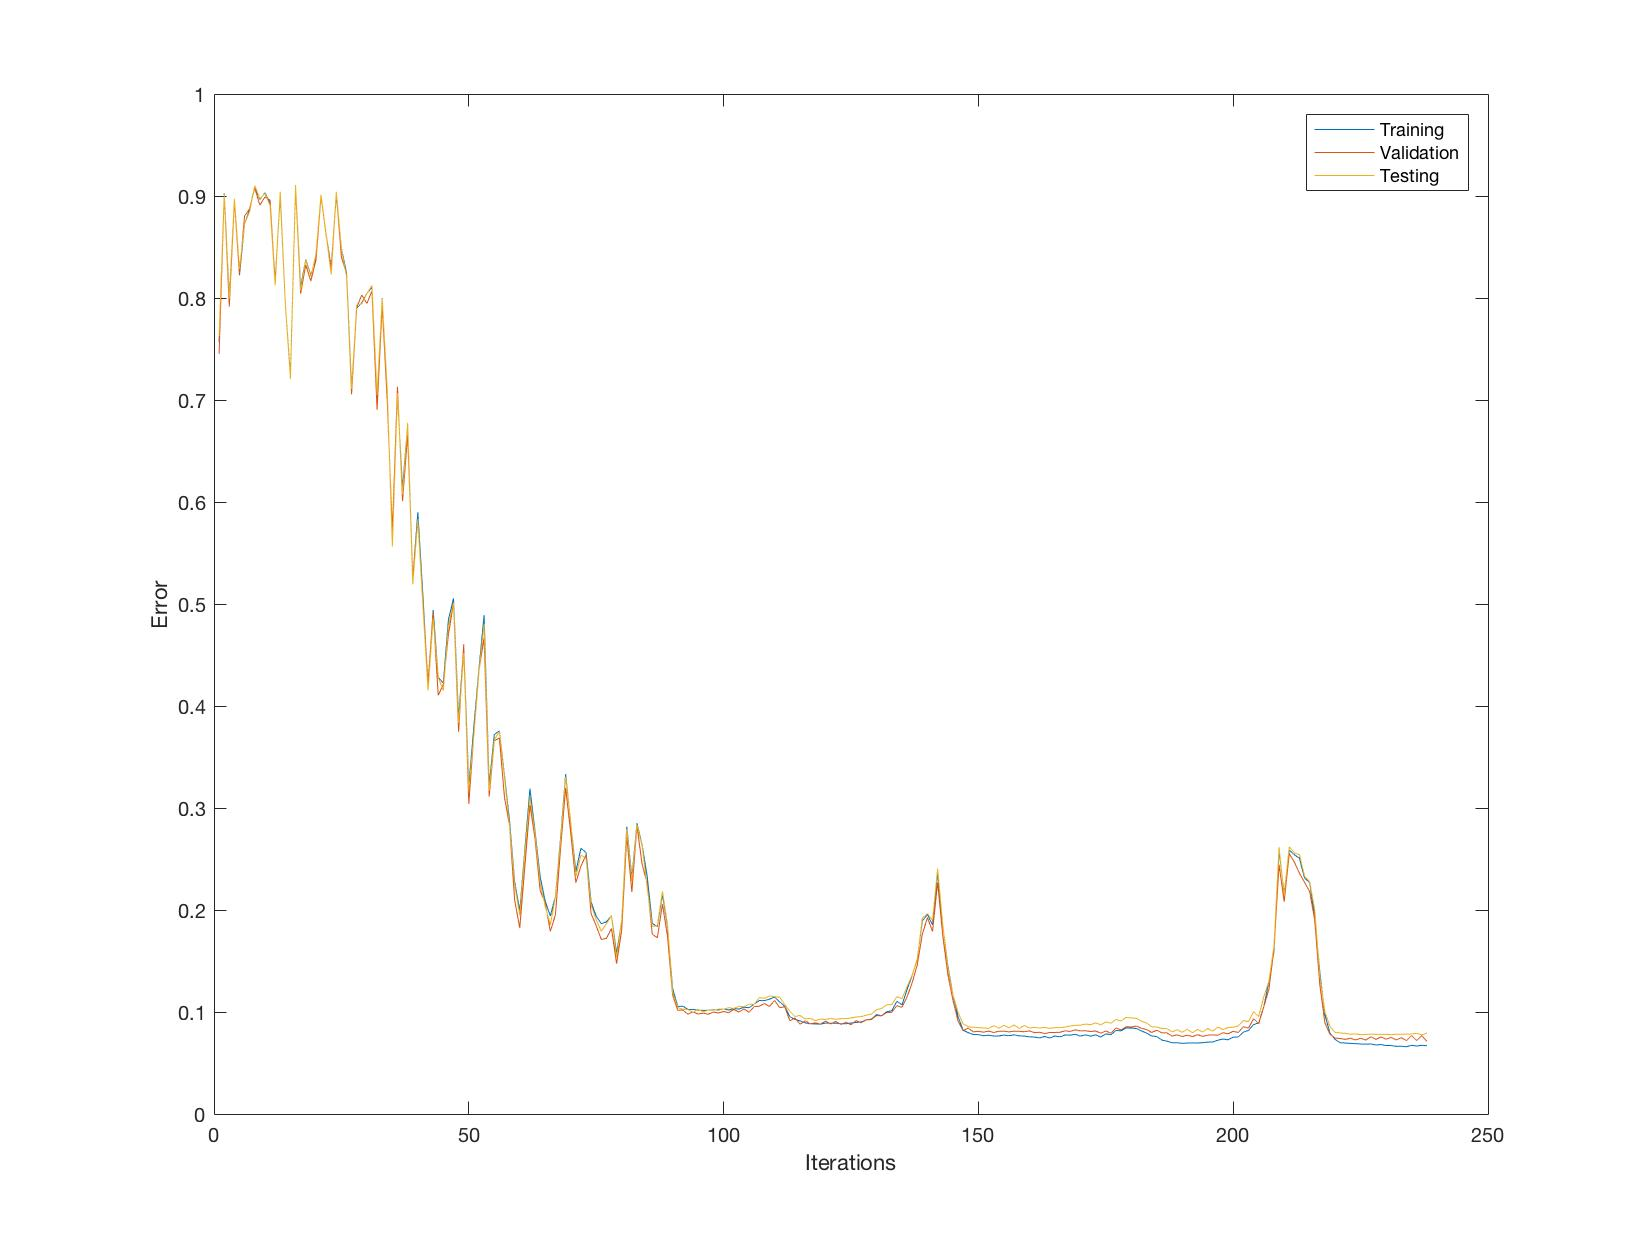
\includegraphics[width=1\textwidth]{full_batch}
  \centering
  \caption{Standard full batch learning}
  \label{fig:3_1}
  \end{figure}

As we can see the learning is very erratic owing to no normalization of the weight updates. Also the accuracy is only 5\% better than the simple softmax regressor we used in the previous assignment.

Also regarding the correctness of the backprop update, we see that the average difference comes out to nearly zero with $\epsilon=0.1$ and $\epsilon=0.01$ and so on (ex. with $\epsilon=0.01$ sum of differences comes out to 0.681 and averaging that over $3*10^{6}$ gives $2*10^{-7}$). Thus it is within the big-O of $\epsilon^{2}$. Hence our backprop implementation is correct.

\subsection{"Tricks of the Trade"}
\begin{enumerate}[label=(\alph*)]

\item \textbf{Mini-batches and update normalization}\\
We used mini-batches of size 125 for convenience instead of 128. The error vs epoch graph for this method is as shown below.

\begin{figure}[H]
  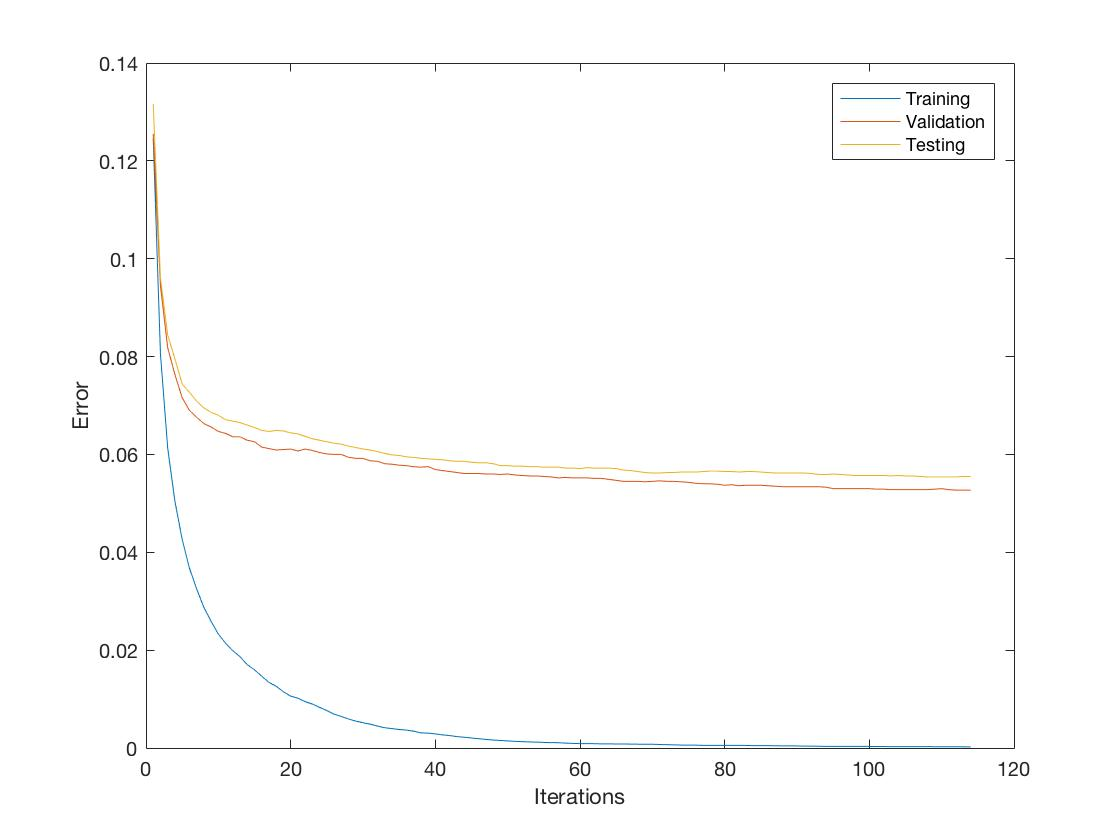
\includegraphics[width=1\columnwidth]{minibatch}
  \centering
  \caption{Mini batch learning}
  \label{fig:4_a}
  \end{figure}
  
We can clearly see a marked improvement in the learning process. It is much more smoother than the previous batch method. We converge to 94.15\% accuracy in just around 120 epochs. Also each epoch only takes 1.33 seconds. Thus mini-batches produce more accurate results than full batch while also being faster.

This is because the mini-batches retain qualities of both stochastic and batch gradient descent. The batch size being small makes updates faster and hence faster learning. Batches also means the updates are meaningful and not affected by random samples. Shuffling the samples also means that with high probability all successive samples belong to different classes. 
  

\item \textbf{$\tanh$ Activation}\\
Retaining the above modifications we further replaced the logistic activations in the hidden layer with $tanh$ activation function. Below we see the error vs epochs graph of the same.

\begin{figure}[H]
  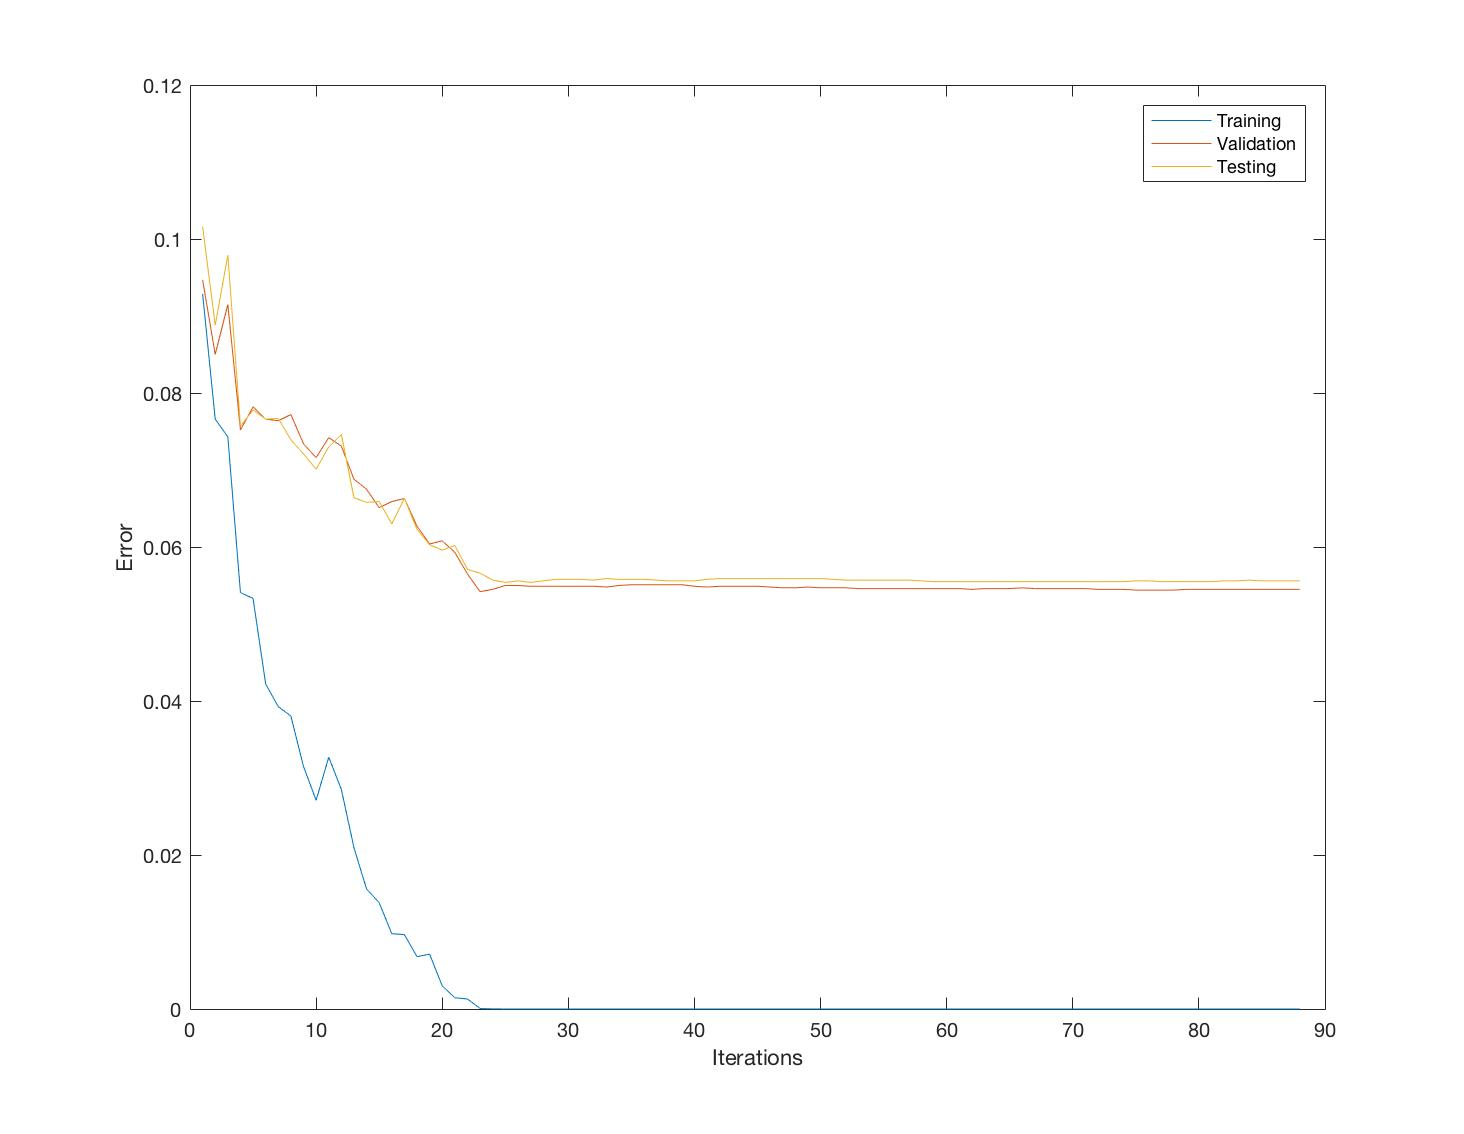
\includegraphics[width=1\columnwidth]{minibatch_tanh}
  \centering
  \caption{Learning using $\tanh$ activation}
  \label{fig:4_b}
  \end{figure}

Again we can see the learning much stabler than the original full batch learning. It achieves a final accuracy of 94.45\% and such the $\tanh$ function is better than the logistic activation function. Also although each epoch takes a little longer at 1.91 seconds seconds per epoch, it converges in around 80 epochs. As such it is still faster than the batch gradient descent.

\item \textbf{Regulating initial weights}\\
Further we initialized the weights using a normal distribution of mean 0 and standard deviation equal to the inverse square root of the number of inputs in the corresponding neuron. Below is the corresponding error vs epoch graph.

\begin{figure}[H]
  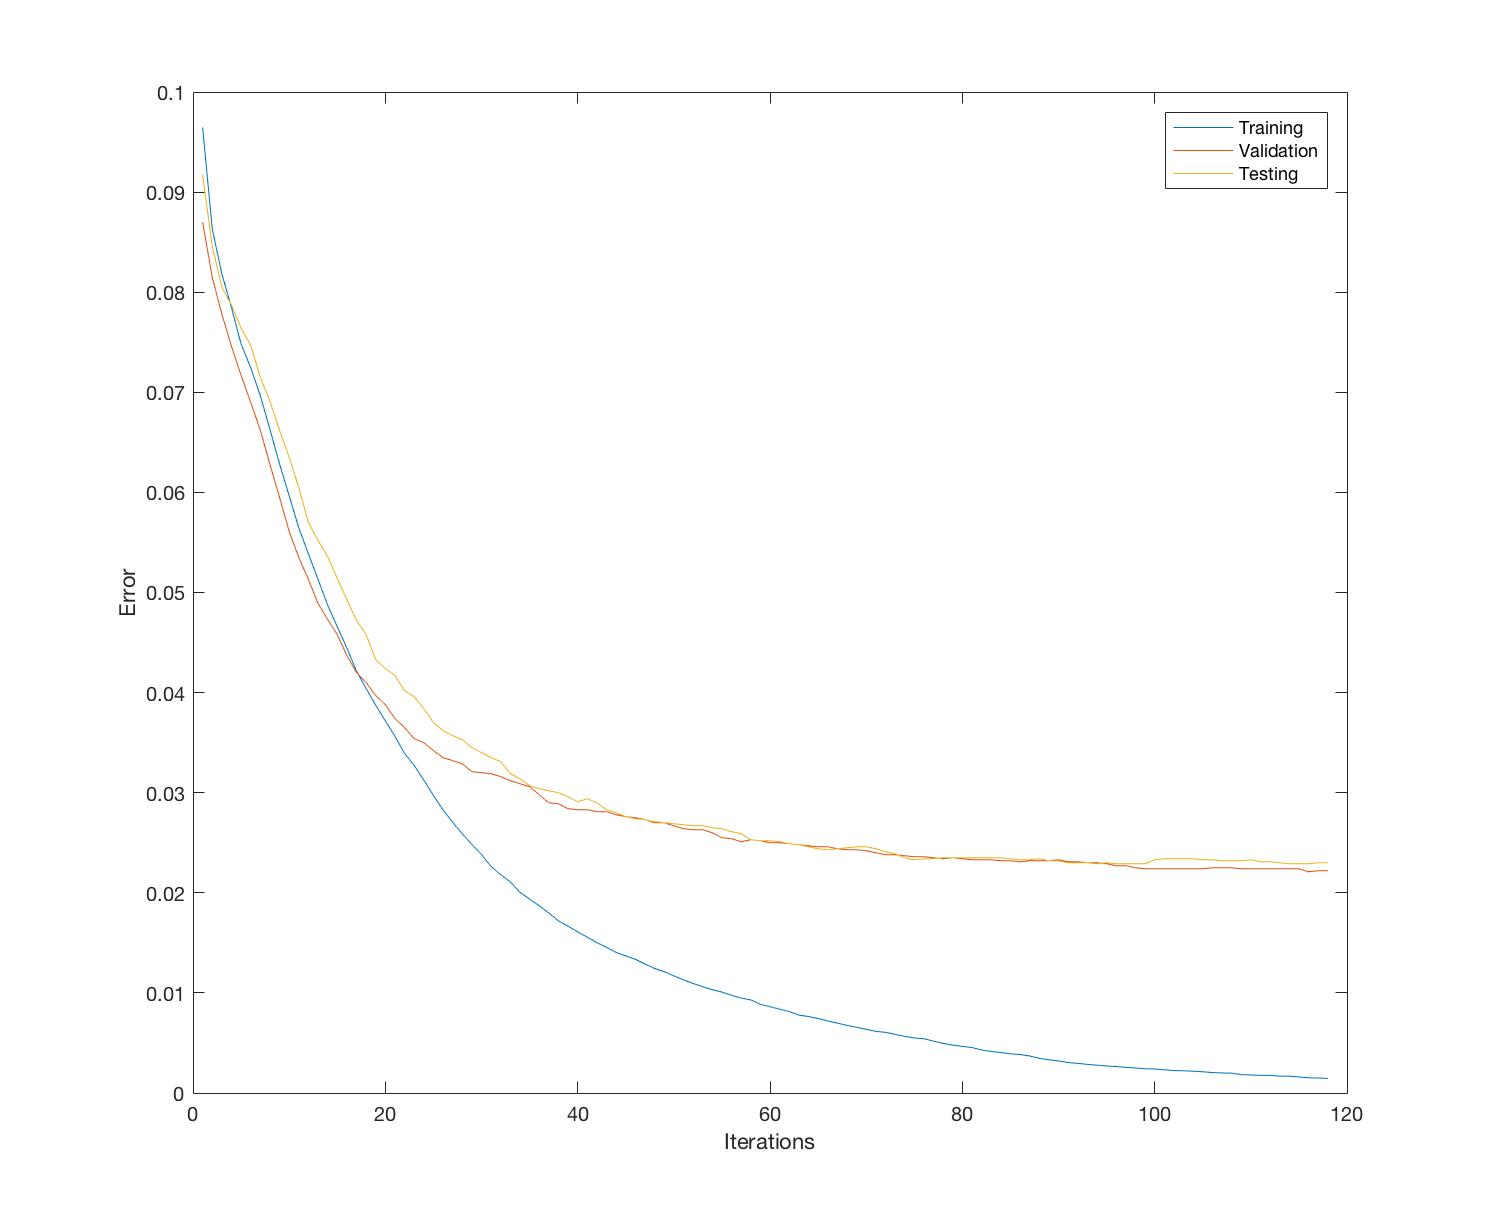
\includegraphics[width=1\columnwidth]{minibatch_tanh_fanin}
  \centering
  \caption{Effect of regulating initial weights}
  \label{fig:4_c}
  \end{figure}

This method reaches a final accuracy of 97.7\% in around 120 epochs and each epoch takes around 1.8 seconds. Thus the regulating the initial weights drastically improves the accuracy while also maintaining training speed.

\item \textbf{Momentum}\\
For the experiments we used a momentum of 0.7. Below we see the graph of error vs epochs while using momentum.

\begin{figure}[H]
  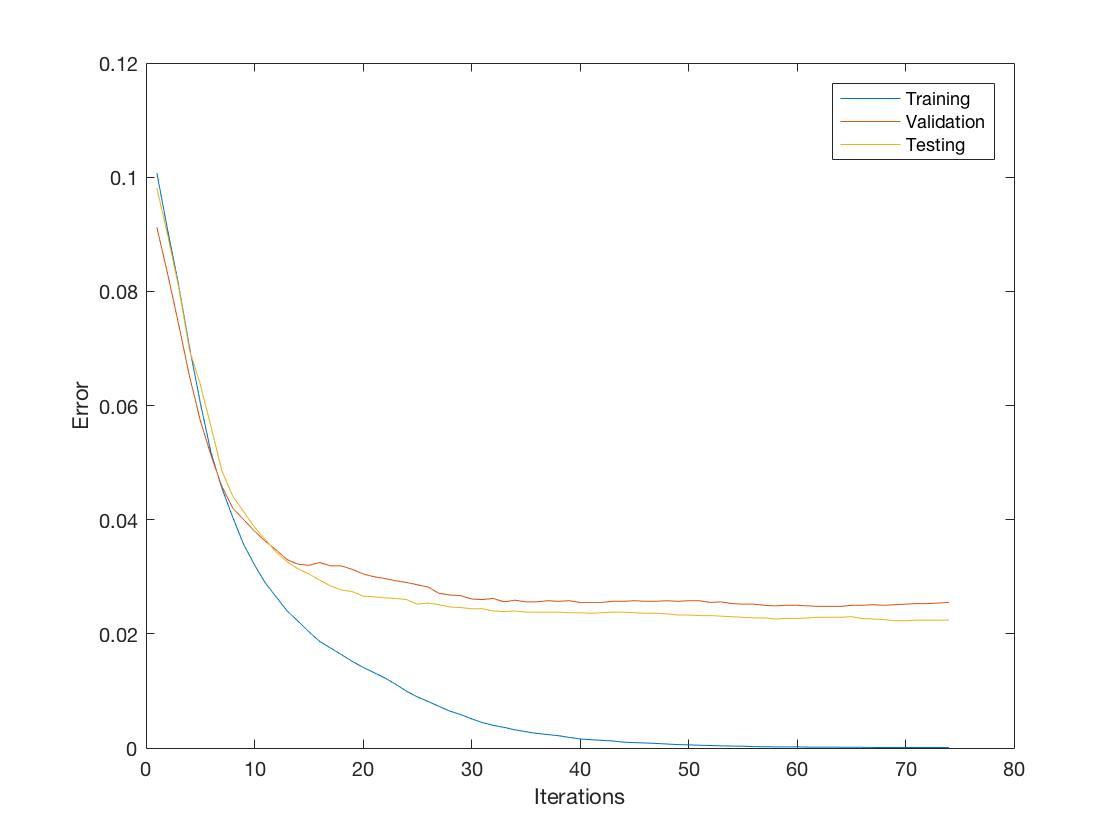
\includegraphics[width=1\columnwidth]{momentum}
  \centering
  \caption{Learning with momentum}
  \label{fig:4_d}
  \end{figure}
We see as expected the graph has a steeper slope meaning that the error goes down much faster. It reaches an accuracy of 97.77\% in a much lesser 80 epochs. Thus again it generates better accuracy in faster time. The time taken per iteration is also around 2.07 seconds.


\end{enumerate}
\subsection{Experiments with network topology}

\begin{enumerate}[label=(\alph*)]

\item \textbf{Doubling number of neurons in hidden layer}\\
From the error vs epochs graph we can see that increasing the number of neurons did not have a profound effect on the training. The final training accuracy was again around 97.72\% after around 100 iterations. Each epoch took around 3.23 seconds to process. As such it only leads to increased training time without much change in accuracy.

\begin{figure}[H]
  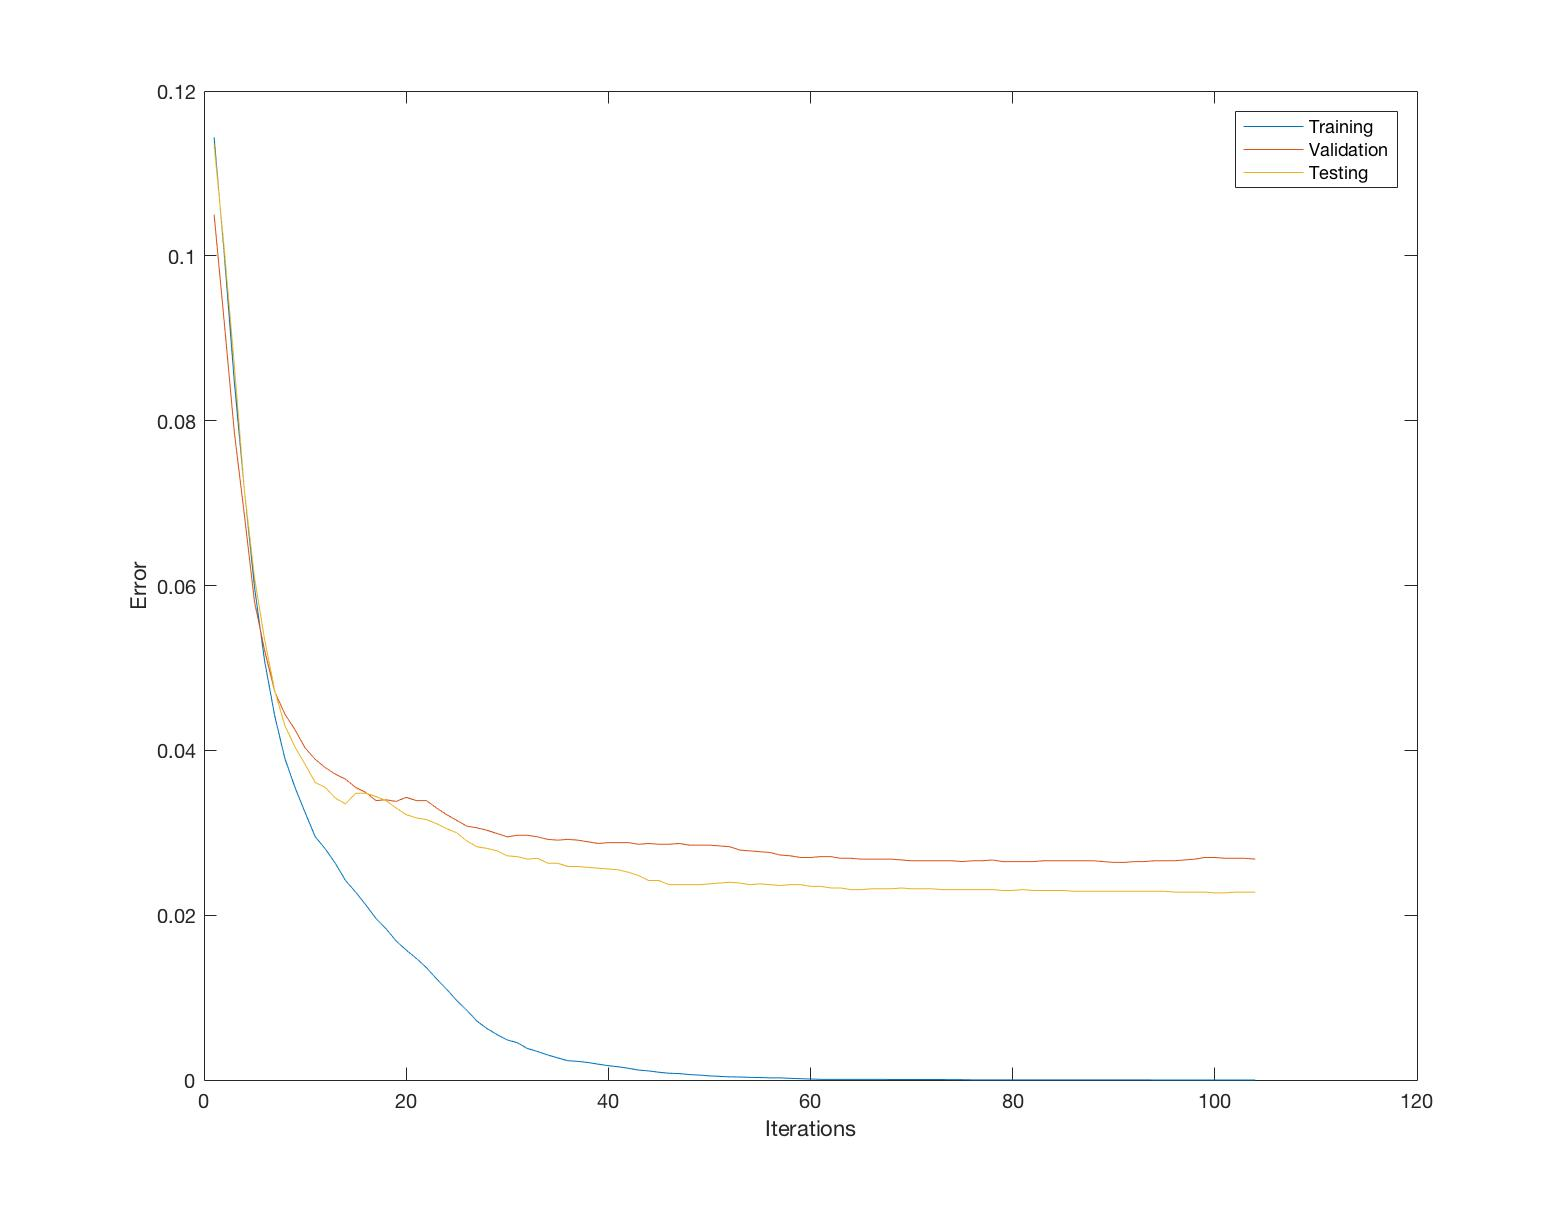
\includegraphics[width=1\columnwidth]{doubleneuron}
  \centering
  \caption{Learning with double the neurons}
  \label{fig:5_a}
  \end{figure}
 
In another case we took 5 neurons to check effect of too low number of neurons. In this case each epoch was much faster at 0.45 seconds per epoch, but the accuracy took a hit. The accuracy achieved in this case was just 85.43\%.

Thus in order to maintain a balance between accuracy and speed, we need to pick an optimum network size which is neither too big nor too small. Big networks lead to larger training times whereas smaller ones give lower accuracy.

\begin{figure}[H]
  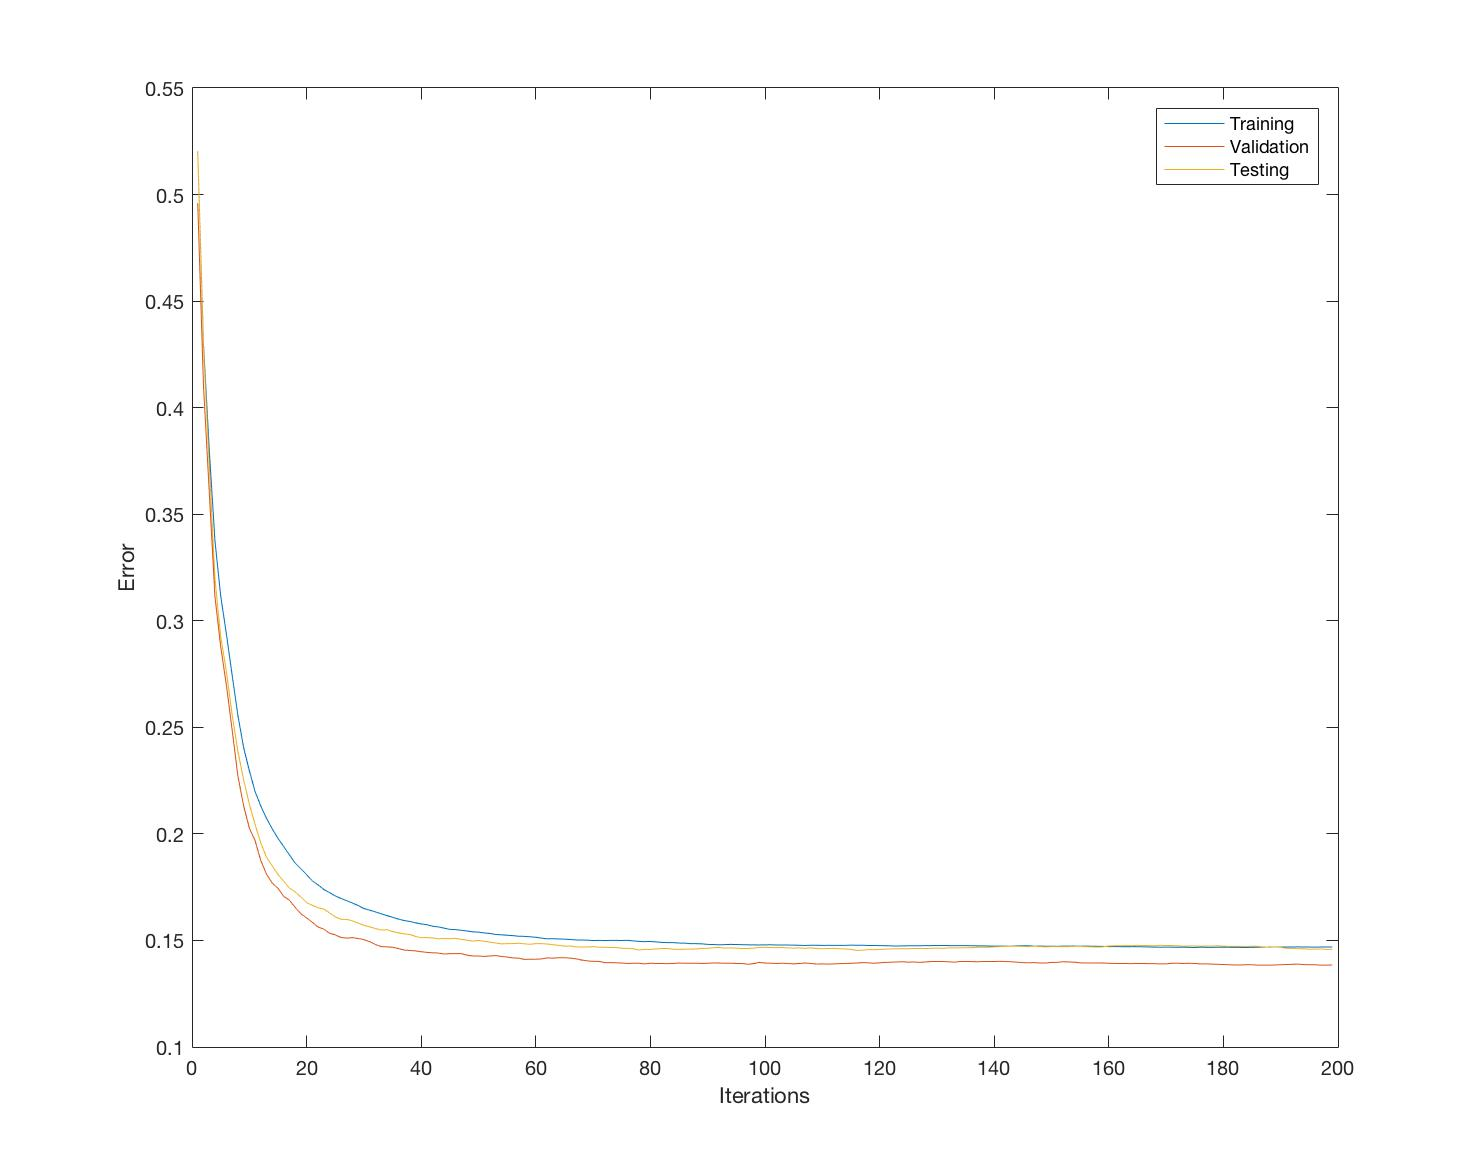
\includegraphics[width=1\columnwidth]{2layer5}
  \centering
  \caption{Learning with 5 neurons}
  \label{fig:5_b}
  \end{figure}
  
\item \textbf{Doubling hidden layers}\\  
As we can see from the figure below, doubling the number of hidden layers again lead to similar accuracies of around 97.7\% as achieved before. But it also takes around 150 epochs and each epoch takes around 3.17 seconds. Thus this is also unnecessary as although it might lead to a slightly better accuracy, it'll take much longer time to reach that. Only very complex classification problems can as such make use of the added complexity provided by an added hidden layer.

\begin{figure}[H]
  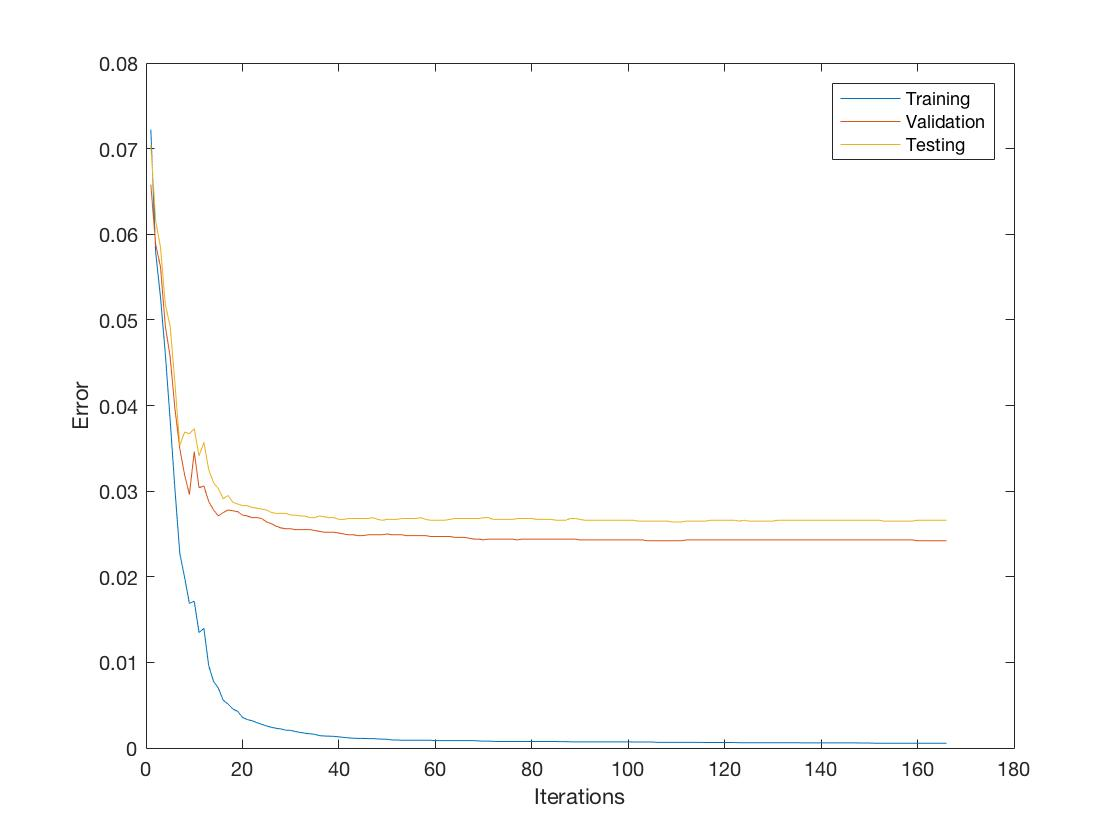
\includegraphics[width=1\columnwidth]{doublelayer}
  \centering
  \caption{Learning with 2 hidden layers}
  \label{fig:6_b}
  \end{figure}
\end{enumerate}

\section{Summary}
\begin{enumerate}[label=(\alph*)]
\item We see that neural networks work much better than the regression techniques we learnt in the last assignment.
\item In particular we see that stochastic gradient descent leads to better learning than batch learning. A mid-way between the two can be in the form of mini-batches.
\item Batch learning leads to low accuracy and the learning itself is also erratic.
\item Mini-batches lead to a balance between fast learning and accurate learning.
\item Normalizing the weight updates leads to faster learning and more accurate networks.
\item A lot also depends on how we initialize our networks. Initializing weights to values, regulated by the number of their inputs leads to faster and more accurate learning.
\item 1.732$ \tanh(\frac{2}{3}x)$ acts as a better activation function than regular logistic function as it is symmetrical around and centered at 0 whereas, the logistic function is always positive.
\item Using momentum further speeds up the learning process and helps avoid plateaus.
\item Needlessly increasing the number of neurons will just add to the overall training time whereas keeping the number too low will lead to lower learning.
\item Increasing the number of layers might increase the accuracy in cases where the added level of complexity is required, but that is rare. So adding the extra layer again adds to training time while the accuracy remains nearly same as the network with single hidden layer.
\end{enumerate}

\section{Contributions}

I, Jean Choi, did 3.\\
I, Ajitesh Gupta, did 4 and 5.\\

\section*{Appendix}
\lstinputlisting[language=MATLAB, caption=MATLAB code to run a 2 layer neural network ]{neural_2layer.m}

\lstinputlisting[language=MATLAB, caption=MATLAB code to run a 3 layer neural network]{neural_3layer.m}

\lstinputlisting[language=MATLAB, caption=MATLAB code to load images from data ]{loadMNISTImages.m}

\lstinputlisting[language=MATLAB, caption=MATLAB code to load labels from data ]{loadMNISTLabels.m}

\lstinputlisting[language=MATLAB, caption=MATLAB code to verify the correctness of the backprop implementation]{checkGradient.m}



%\end{appendices}

\printbibliography
\end{document}
